\section{Lasso estimatoren og dens generaliseringer}
\begin{frame}{Lasso estimatoren}
\textit{The Least Absolute Shrinkage Selection Operator} (lasso) løser optimeringsproblemet
\begin{align*}
\widehat{\boldsymbol{\beta}}^\text{lasso} = \argmin_{\boldsymbol{\beta} \in \R^p} \cbr{\sum_{i=1}^n \del{y_i - \sum_{j=1}^p x_{ij} \beta_j}^2}, \ \text{u.h.t. at } \sum_{j=1}^p \vert \beta_j \vert \leq t,
\end{align*} 
som kan omskrives til et lagrange problem
\begin{align*}
\widehat{\boldsymbol{\beta}}^\text{lasso} = \argmin_{\boldsymbol{\beta} \in \R^p} \cbr{ \Vert \mathbf{y} - \mathbf{X} \boldsymbol{\beta} \Vert_2^2 + \lambda \Vert \boldsymbol{\beta} \Vert_1},
\end{align*}
hvor \(\lambda \geq 0\).
Ridge regression estimatoren findes ud fra
\begin{align*}
\widehat{\boldsymbol{\beta}}^\text{ridge} &= \argmin_{\boldsymbol{\beta} \in \R^p} \cbr{ \Vert \mathbf{y} - \mathbf{X} \boldsymbol{\beta} \Vert_2^2 + \lambda \Vert \boldsymbol{\beta} \Vert_2^2} \\
&= \del{\mathbf{X}^T \mathbf{X} + \lambda \mathbf{I}_p}^{-1} \mathbf{X}^T \mathbf{y}.
\end{align*} 
\end{frame}

\begin{frame}{Lasso estimatoren}
\begin{figure}[H]
\centering
\begin{minipage}{0.4\linewidth}
\scalebox{0.6}{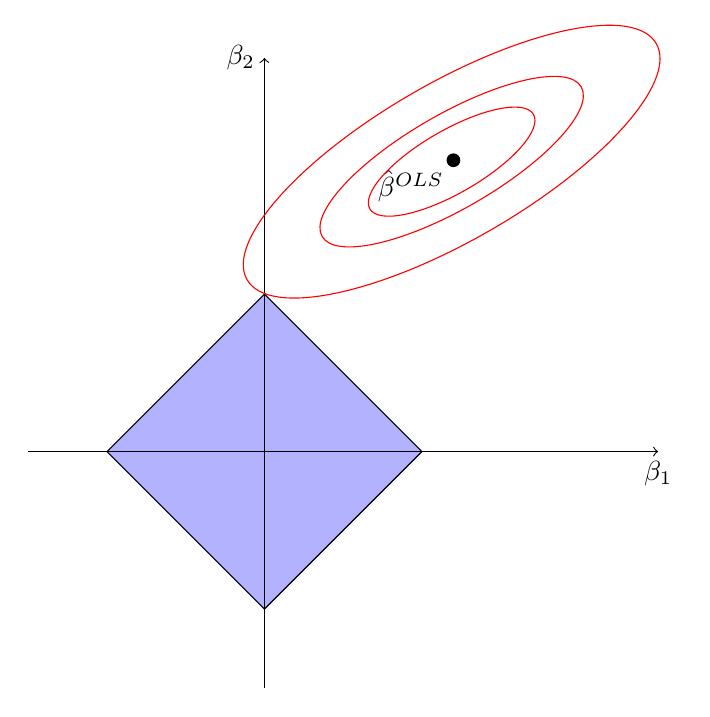
\begin{tikzpicture}
\draw [fill] (2.4,3.7) circle [radius=0.08];
\node [below left] (a) at (2.4,3.7) {$\hat{\beta}^\text{OLS}$};
\draw (-2,0) -- (0,2) -- (2,0)-- (0,-2) -- (-2,0)[fill = blue!30];
\draw [<-] (0,5) node [left] {$\beta_2$}-- (0,-3);
\draw[<-] (5,0) node [below] {$\beta_1$} -- (-3,0);
\begin{scope}[rotate = 30, red]
\clip[draw] (3.9,2) ellipse (3cm and 1cm);
\clip[draw] (3.9,2)ellipse (1.9 cm and 0.6 cm); 
\clip[draw] (3.9,2) ellipse (1.2 cm and 0.4 cm);
\end{scope}
\end{tikzpicture}}
\end{minipage}
\hspace{0.2cm}
\begin{minipage}{0.4\linewidth}
\scalebox{0.6}{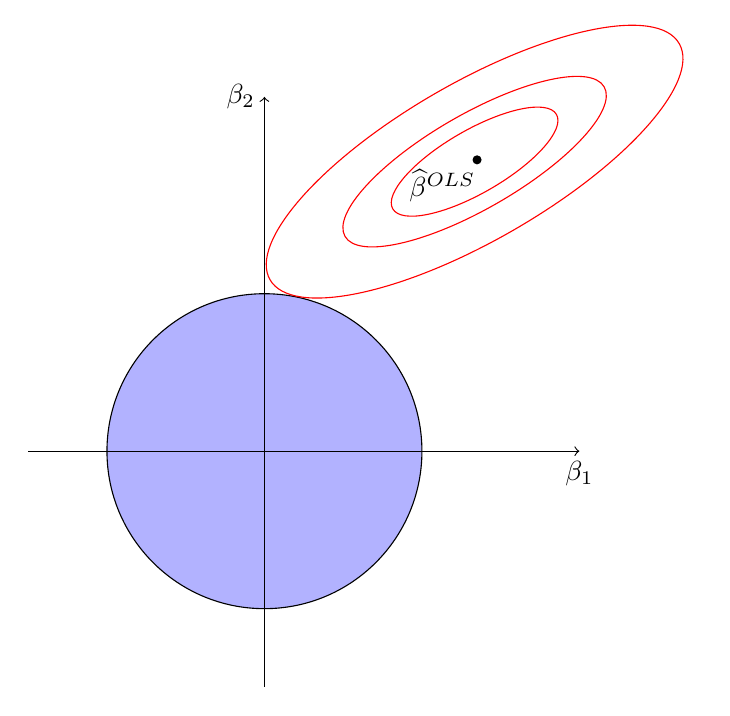
\begin{tikzpicture}
\draw [fill] (2.7,3.7) circle [radius=0.05];
\node [below left] (a) at (2.8,3.7) {$\widehat{\boldsymbol{\beta}}^\text{OLS}$};
\draw (0,0) circle (2cm) [fill= blue!30];
\draw [<-] (0,4.5) node [left] {$\beta_2$}-- (0,-3);
\draw[<-] (4,0) node [below] {$\beta_1$} -- (-3,0);
\begin{scope}[rotate = 30, red]
\clip[draw] (4.15,1.85) ellipse (3cm and 1cm);
\clip[draw] (4.15,1.85)ellipse (1.9 cm and 0.6 cm); 
\clip[draw] (4.15,1.85) ellipse (1.2 cm and 0.4 cm);
\end{scope}
\end{tikzpicture}}
\end{minipage}
\caption{Estimations illustration for lasso (venstre) og ridge regression (højre). 
De blå arealer er betingelsesområderne $\vert \beta_1 \vert+\vert \beta_2 \vert \leq t$ og $\beta_1^2+\beta_2^2 \leq t^2$, mens de røde ellipser er konturkurver for SSR. Konturkurverne har centrum i OLS estimatoren, $\widehat{\boldsymbol{\beta}}^\text{OLS}$.}
\end{figure}
\end{frame}



\begin{frame}{Generaliseringer af lasso estimatoren}{Naiv elastisk net}
Selvom lasso har vist succes i mange tilfælde, har den også nogle begrænsninger:
\begin{itemize}
\item Hvis \(p>n\), da udvælger lasso højst \(n\) variable.
\item Hvis der eksisterer en gruppe af variable med høj parvis korrelation, da vil lasso blot udvælge én variabel fra denne gruppe og denne variabel udvælges tilfældigt.
\end{itemize}

Naiv elastisk net løser optimeringsproblemet
\begin{align*}
\widehat{\boldsymbol{\beta}}^\text{naivEN} =\argmin_{\boldsymbol{\beta} \in \R^p} \cbr{ \Vert \mathbf{y} - \mathbf{X} \boldsymbol{\beta} \Vert_2^2 + \lambda \sbr{\frac{1}{2}(1- \alpha) \Vert \boldsymbol{\beta} \Vert_2^2 + \alpha \Vert \boldsymbol{\beta} \Vert_1}}. 
\end{align*}
\begin{itemize}
\item Hvis $\alpha=0$, da reduceres strafleddet til den kvadrerede $\ell_2$-norm svarende til strafleddet for ridge regression.
\item Hvis $\alpha=1$ reduceres strafleddet til $\ell_1$-normen svarende til strafleddet for lasso.
\end{itemize}
\end{frame}

\begin{frame}{Generaliseringer af lasso estimatoren}{Group lasso}
Antag variablerne er opdelt i \(J\) grupper, hvor \(p_j\) er antallet af variable i gruppe \(j\). \\

%Lad \(\mathbf{z}_j\) og \(\boldsymbol{\theta}_j\) være \(p_j \times 1\) vektorer som repræsenterer prædiktorerne og deres koefficienter i gruppe \(j\) for \(j = 1, \ldots, J\).
Group lasso løser følgende optimeringsproblem
\begin{align*}
\widehat{\boldsymbol{\theta}}_j^{\text{group lasso}} = \argmin_{\boldsymbol{\theta}_1, \ldots, \boldsymbol{\theta}_J} \cbr{\frac{1}{2} \Vert \mathbf{y} - \sum_{j=1}^J \mathbf{Z}_j \boldsymbol{\theta}_j \Vert_2^2 + \lambda \sum_{j=1}^J \sqrt{p_j} \Vert \boldsymbol{\theta}_j \Vert_2}.
\end{align*}
\begin{itemize}
\item Alle indgange i $\widehat{\boldsymbol{\theta}}_j^\text{group lasso}$ vil være lig nul eller ikke-nul afhængig af \(\lambda\).
\item Når $p_j=1$, da har vi, at $\Vert \boldsymbol{\theta}_j \Vert_2 = \vert \boldsymbol{\theta}_j \vert$, således at alle grupper består af én prædiktor, dermed reduceres optimeringsproblemet til standard lasso.
\end{itemize}
\end{frame}
%
\begin{frame}{Generaliseringer af lasso estimatoren}{Adaptive lasso}
Ideen bag adaptive lasso er at tildele koefficienterne individuelle straffe, istedet for at alle koefficienter straffes ligeligt.

Antag \(\widetilde{\boldsymbol{\beta}}\) er rod-n konsistent til \(\boldsymbol{\beta}^*\). Vælg \(\gamma >0\), da er adaptive lasso estimaterne givet ved
\begin{align*}
\widehat{\boldsymbol{\beta}}^\text{AL} = \argmin_{\boldsymbol{\beta} \in \R^p} \cbr{ \Vert \mathbf{y} - \mathbf{X} \boldsymbol{\beta} \Vert_2^2 + \lambda \sum_{j=1}^p \frac{ \vert \beta_j \vert}{\vert \widetilde{ \beta}_j \vert^\gamma}}.
\end{align*}
\begin{itemize}
\item opfylder orakelegenskaberne, hvilket betyder, at variabeludvælgelsen er konsistent.
\end{itemize}
%\begin{itemize}
%\item Lad $\pazocal{A}_n^\text{AL} = \cbr{j: \widehat{\beta}_j^\text{AL} \neq 0}$ betegne den aktive mængde for adaptive lasso estimatoren.
%\end{itemize} 
%Sætning \\
%Antag $\frac{\lambda_n}{\sqrt{n}} \rightarrow 0$ og $\lambda_n n^\frac{\gamma - 1}{2} \rightarrow \infty$, da opfylder adaptive lasso orakelegenskaberne:
%\begin{itemize}
%\item Konsistent variabeludvælgelsen: $\lim_{n \rightarrow \infty} \mathbb{P}(\pazocal{A}_n^\text{AL}=\pazocal{A})=1$.
%\item Asymptotisk normalitet: $\sqrt{n}\left( \widehat{\boldsymbol{\beta}}_\pazocal{A}^{\text{AL}}-\boldsymbol{\beta}_\pazocal{A}^* \right) \overset{d}{\rightarrow} N(\textbf{0},\sigma^2 \boldsymbol{C}_{11}^{-1}).$
%\end{itemize} 
\end{frame}

%%% Local Variables:
%%% mode: latex
%%% TeX-master: "../beamer"
%%% End:
